%%%%%%%%%%%%%%%%%%%%%%%%%%%%%%%%%%%%%%%%%%%%%%%%%%%%%%%%%%%%%%%%%%%%%%%%%%%%%%%%%%%%%%%%%%%%%%%%%
%
% Document:      DiskKinematicsVrad.tex
% Author:        Anthony Brown
% Revision:      1
% Last Updated:  2020.10.21
% First Created: 2020.10.21
% Title:         Milky Way disk kinematics: radial velocity
% Description:   Schematic for calculating the radial velocity of a given star in the Milky Way with
%                respect to the Sun.
%
%%%%%%%%%%%%%%%%%%%%%%%%%%%%%%%%%%%%%%%%%%%%%%%%%%%%%%%%%%%%%%%%%%%%%%%%%%%%%%%%%%%%%%%%%%%%%%%%%

\documentclass{article}

\usepackage{times,layouts}
\usepackage{tikz,hyperref,amsmath}
\usepackage{macros-agabrown}
\usetikzlibrary{arrows,shapes,decorations.shapes,shapes.arrows}
\usetikzlibrary{positioning,backgrounds,calc,shadings}
\usetikzlibrary{angles,quotes,math}

\usepackage{geometry}
\geometry{hmargin=5pt, vmargin=5pt}

\definecolor{softblue}{rgb}{0.5, 0.5, 1.0}
\definecolor{softyellow}{rgb}{1.0, 1.0, 0.3}
\definecolor{softcyan}{rgb}{0.5, 1.0, 1.0}
\definecolor{softgreen}{rgb}{0.5, 1.0, 0.5}
\definecolor{softmagenta}{rgb}{1.0, 0.5, 1.0}
\definecolor{softorange}{rgb}{1.0, 0.9375, 0.5}
\definecolor{gaiared}{rgb}{0.866666666667, 0, 0.23137254902}
\definecolor{gaiareddark}{rgb}{0.51372549, 0.03529412, 0.16862745}

\definecolor{dpacyellow}{rgb}{0.97254902, 0.76862745, 0.}
\definecolor{dpacpetrol}{rgb}{0.24313725, 0.45490196, 0.55294118}

\newcommand\showpage{%
  \setlayoutscale{0.5}\setlabelfont{\tiny}\printheadingsfalse\printparametersfalse
  \currentpage\pagedesign}
\newcommand\rood[1]{\color{red}#1}

\hypersetup{pdftitle={Milky Way disk kinematics: radial velocity}, pdfsubject={Schematic for calculating
the radial velocity of a given star in the Milky Way wuth respect to the Sun.}, pdfauthor={Anthony
Brown}}

\tikzstyle{lijn}=[shorten >=2pt, shorten <=2pt, line width=1pt]
\tikzstyle{vect}=[->, shorten >=0pt, shorten <=0pt, >=stealth', line width=1pt]
\tikzstyle{vectrev}=[<-, shorten >=2pt, shorten <=2pt, >=stealth', line width=1pt]

%\newdimen\distance
%\setlength{\distance}{6cm}
\newcommand\distance{6}
%\newdimen\rsun
%\setlength{\rsun}{8.2cm}
\newcommand\dsun{8.2}
\newdimen\vrot
\setlength{\vrot}{2.0cm}
\newcommand\galon{20}

\begin{document}
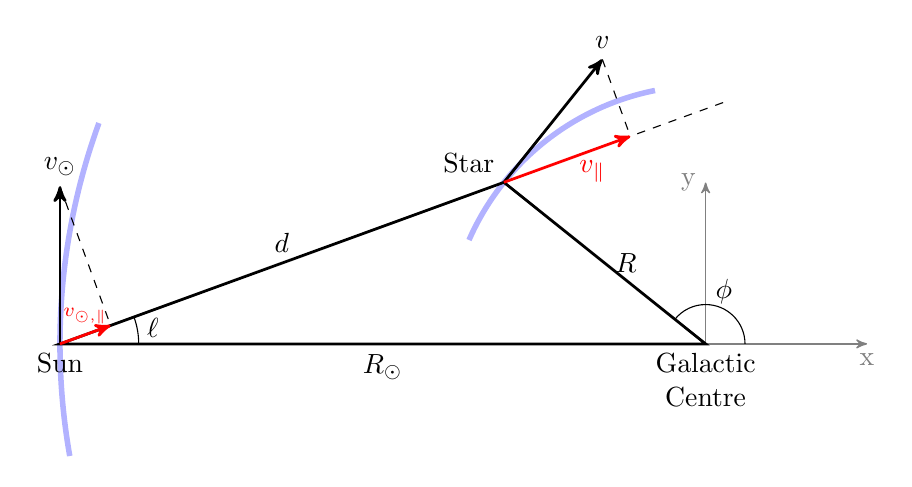
\begin{tikzpicture}
  \coordinate (sun) at (0,0);
  \coordinate (gc) at (\dsun,0);
  \coordinate (gcx) at ($(gc)+(1,0)$);
  \coordinate (star) at (\galon:\distance);
  \tikzmath{
    real \rstar;
    real \anglebeta;
    \rstar = sqrt(\distance*\distance+\dsun*\dsun-2*\distance*\dsun*cos(\galon));
    \anglebeta = 180-asin(\distance/\rstar*sin(\galon));
  }

  \draw[vect, line width=0.5pt, color=black!50!white] (\dsun,0) -- ++(0.25*\dsun, 0) node[below]{\vect{x}};
  \draw[vect, line width=0.5pt, color=black!50!white] (\dsun,0) -- ++(0, 0.25*\dsun) node[left]{\vect{y}};

  \draw[color=blue!30!white, line width=2pt] (gc) ++(190:\dsun) arc (190:160:\dsun);
  \draw[color=blue!30!white, line width=2pt] (gc) ++(\anglebeta+15:\rstar) arc
  (\anglebeta+15:\anglebeta-40:\rstar);

  \draw[dashed] (sun) -- ($(sun)!1.5!(star)$);
  \draw[draw=none] (gc) -- (sun) -- (star) pic [draw=black, angle radius=10mm, "$\ell$", angle
  eccentricity=1.2] {angle=gc--sun--star};
  %\draw[draw=none] (sun) -- (star) -- (gc) pic [draw=black, angle radius=5mm, "$\alpha$", angle
  %eccentricity=1.3] {angle=sun--star--gc};
  \draw[draw=none] (gcx) -- (gc) -- (star) pic [draw=black, angle radius=5mm, "$\phi$", angle
  eccentricity=1.4] {angle=gcx--gc--star};

  \draw[lijn] (sun) -- node[below]{$R_\odot$} (gc) -- node[right]{$R$} (star) --
  node[above]{$d$} cycle;
  \coordinate (a) at ($(sun)!\vrot!90:(gc)$);
  \coordinate (aproj) at ($(sun)!(a)!(star)$);
  \draw[vect] (sun) -- (a) node[above] {$\vectbar{v}_\odot$};
  \draw[dashed] (a) -- (aproj);
  \draw[vect, color=red] (sun) -- node[above, font=\scriptsize]{$v_{\odot,\parallel}$} (aproj);

  \coordinate (c) at ($(star)!\vrot!90:(gc)$);
  \coordinate (cproj) at ($(sun)!(c)!(star)$);
  \draw[vect] (star) -- (c) node[above] {$\vectbar{v}$};
  \draw[dashed] (c) -- (cproj);
  \draw[vect, color=red] (star) -- node[below, pos=0.7]{$v_\parallel$} (cproj);

  \node at (sun.south) [anchor=north]{Sun};
  \node at (star.west) [anchor=south east]{Star};
  \node at (gc.south) [anchor=north, text width=1.5cm, text badly centered]{Galactic Centre};
\end{tikzpicture}
\end{document}
